\chapter{Конструкторская часть}

\section{Последовательность действий}

На рисунке~\ref{img:alg:idef0-1} представлена последовательность действий, выполняемых при загрузке модуля, а на рисунке~\ref{img:alg:idef0-2} --- при выгрузке модуля.

\begin{figure}[h]
	\centering
	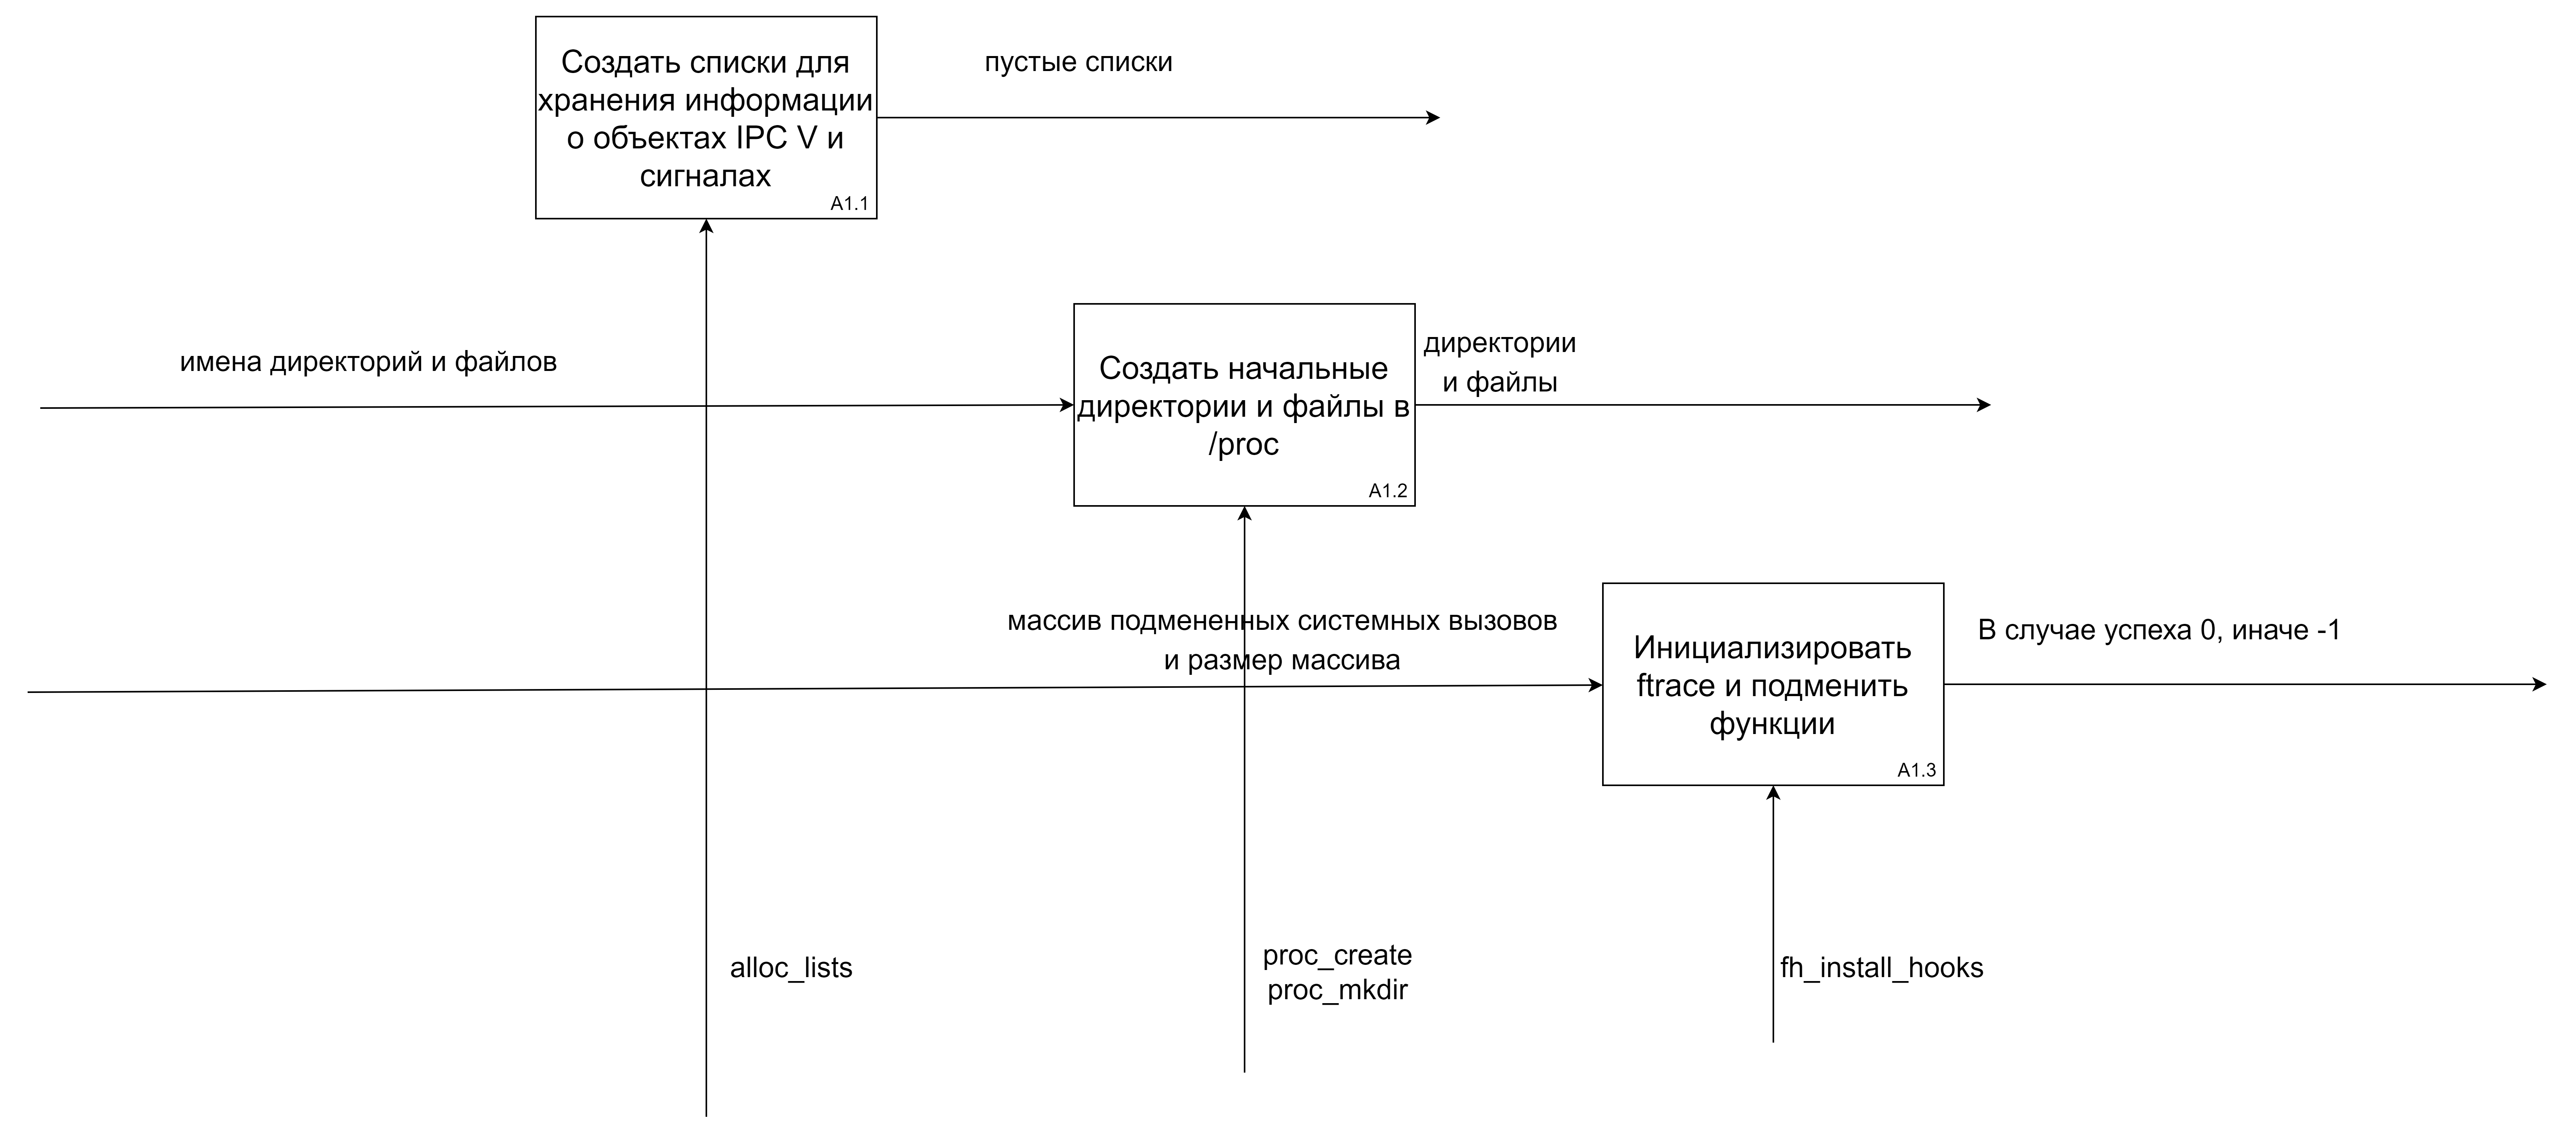
\includegraphics[height=0.3\textheight]{img/idef0-1.png}
	\caption{Последовательность действий при загрузке модуля}
	\label{img:alg:idef0-1}
\end{figure}

\begin{figure}[h]
	\centering
	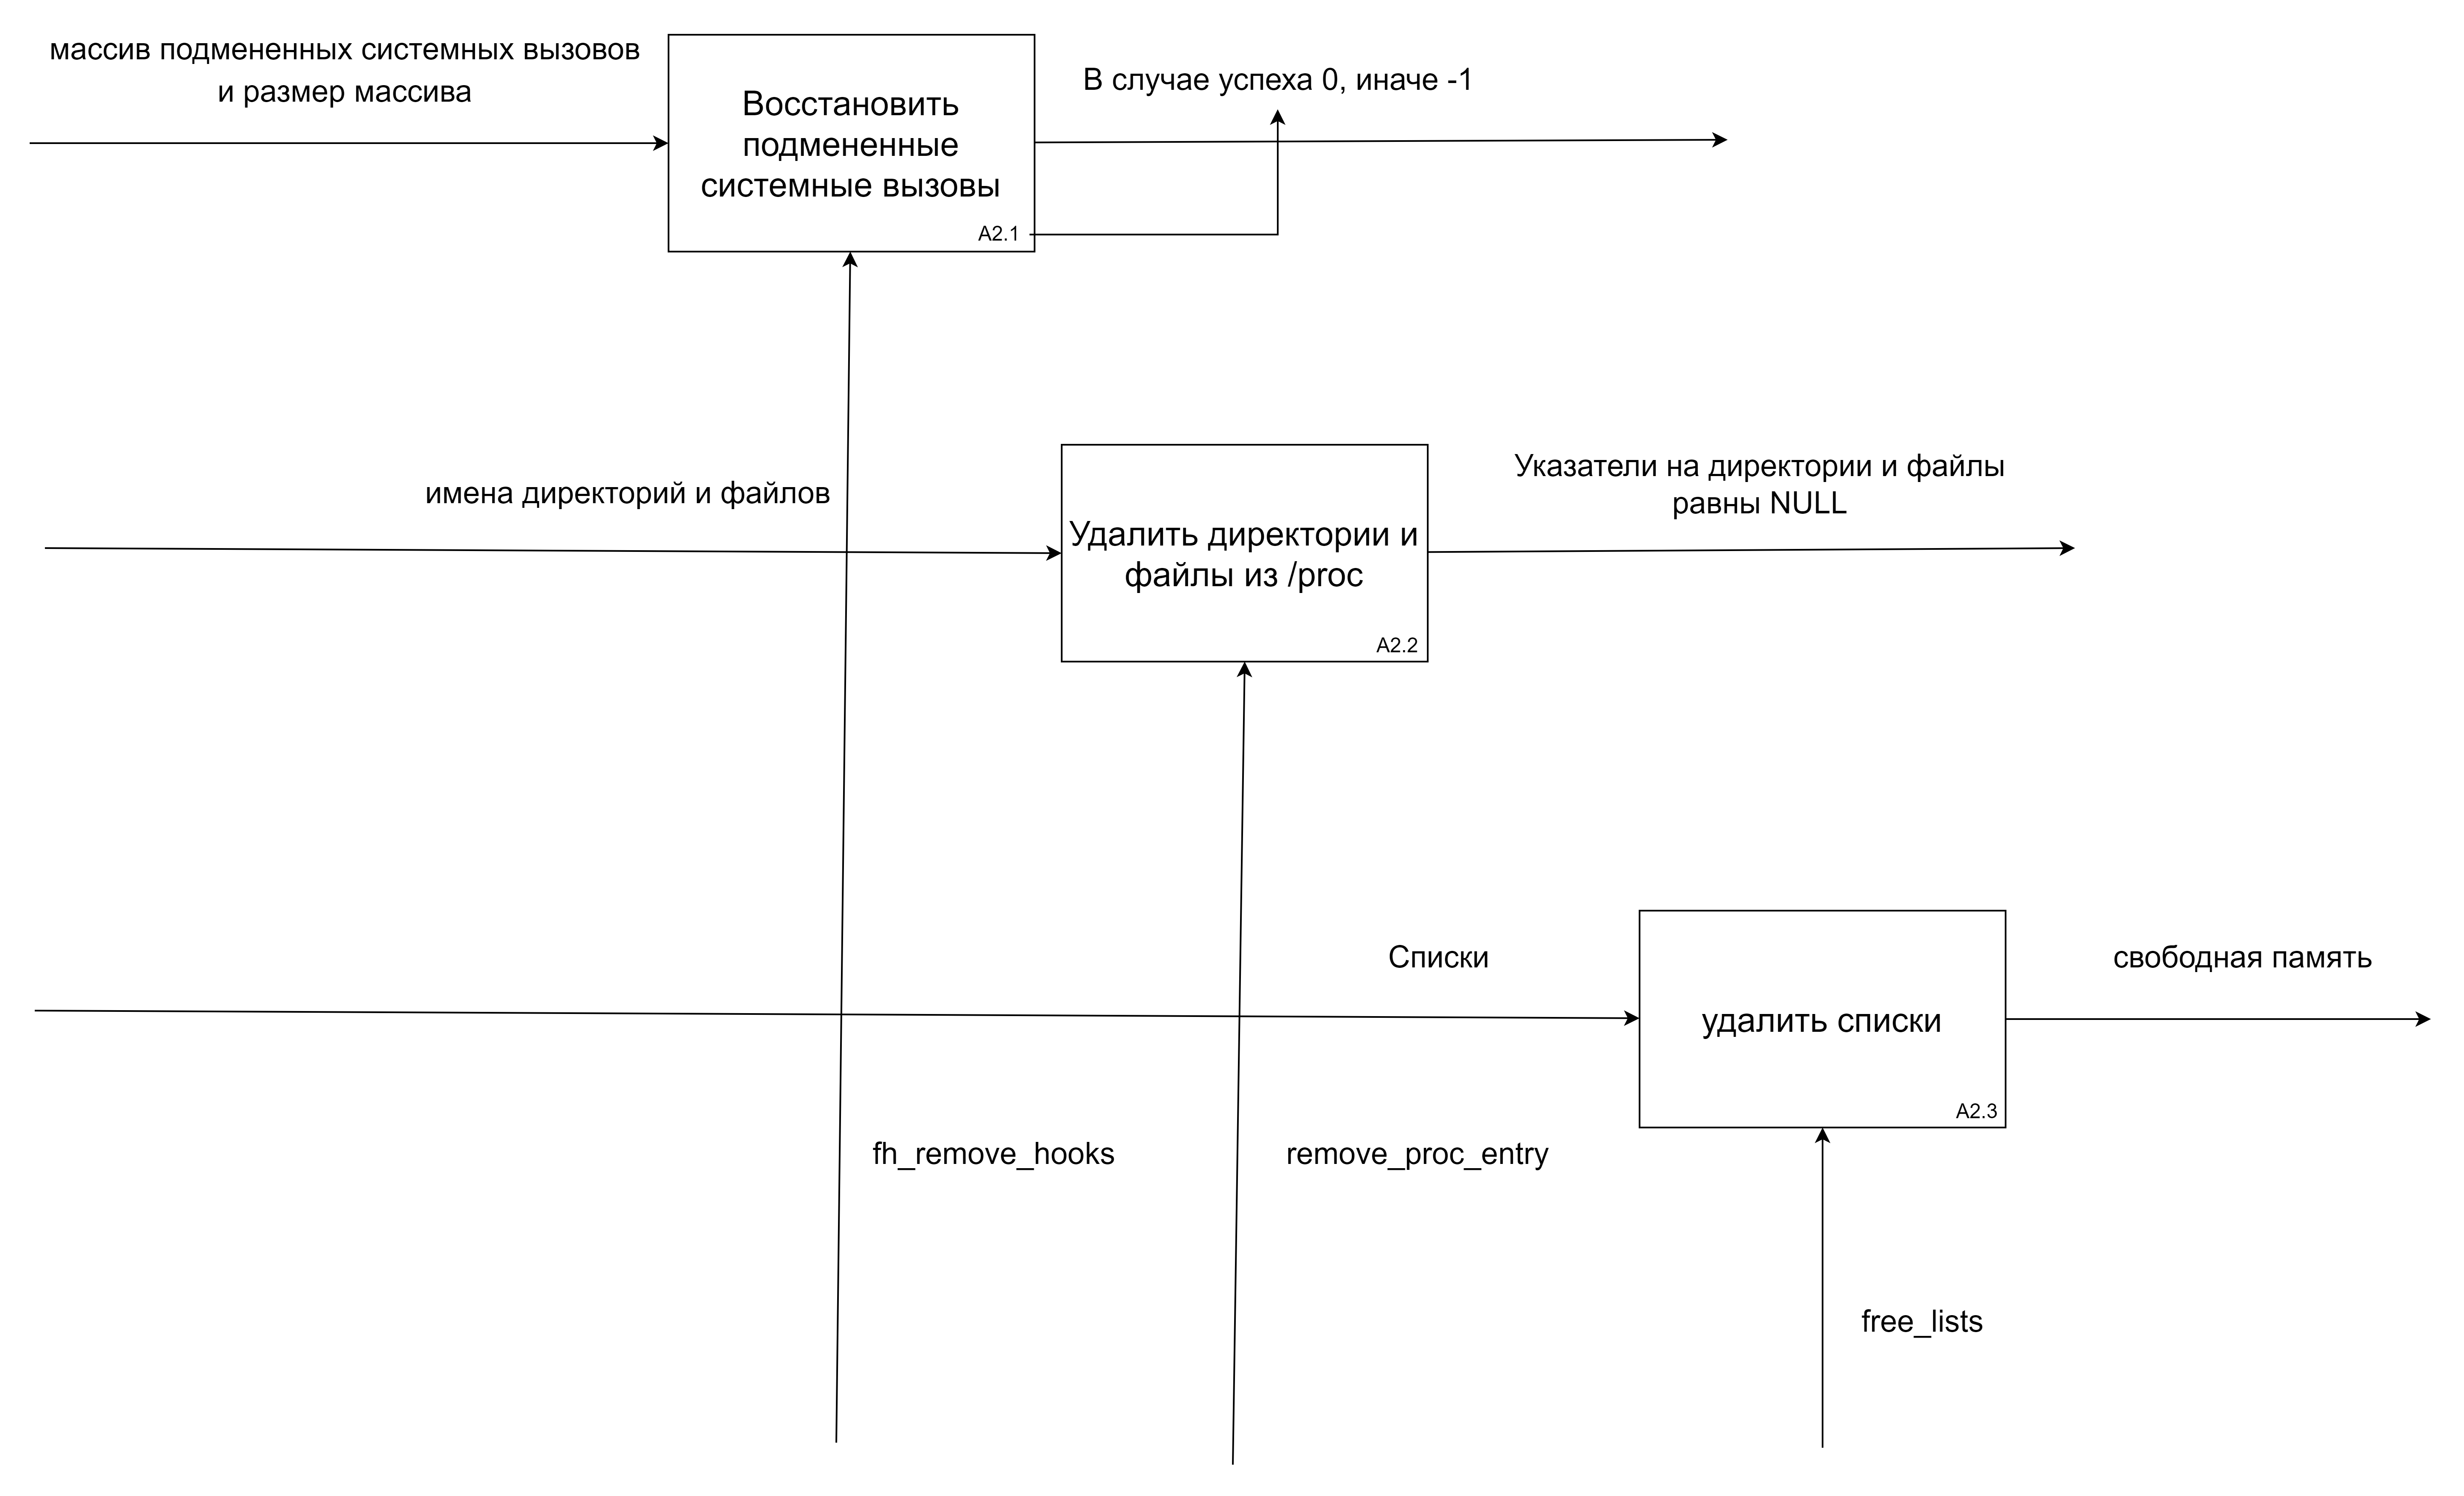
\includegraphics[height=0.3\textheight]{img/idef0-2.png}
	\caption{Последовательность действий при выгрузке модуля}
	\label{img:alg:idef0-2}
\end{figure}


\clearpage

\section{Разработка алгоритмов}

На риснуке~\ref{img:alg:ftrace} представлены схемы алгоритмов загрузки и выгрузки модуля.

\begin{figure}[h]
	\centering
	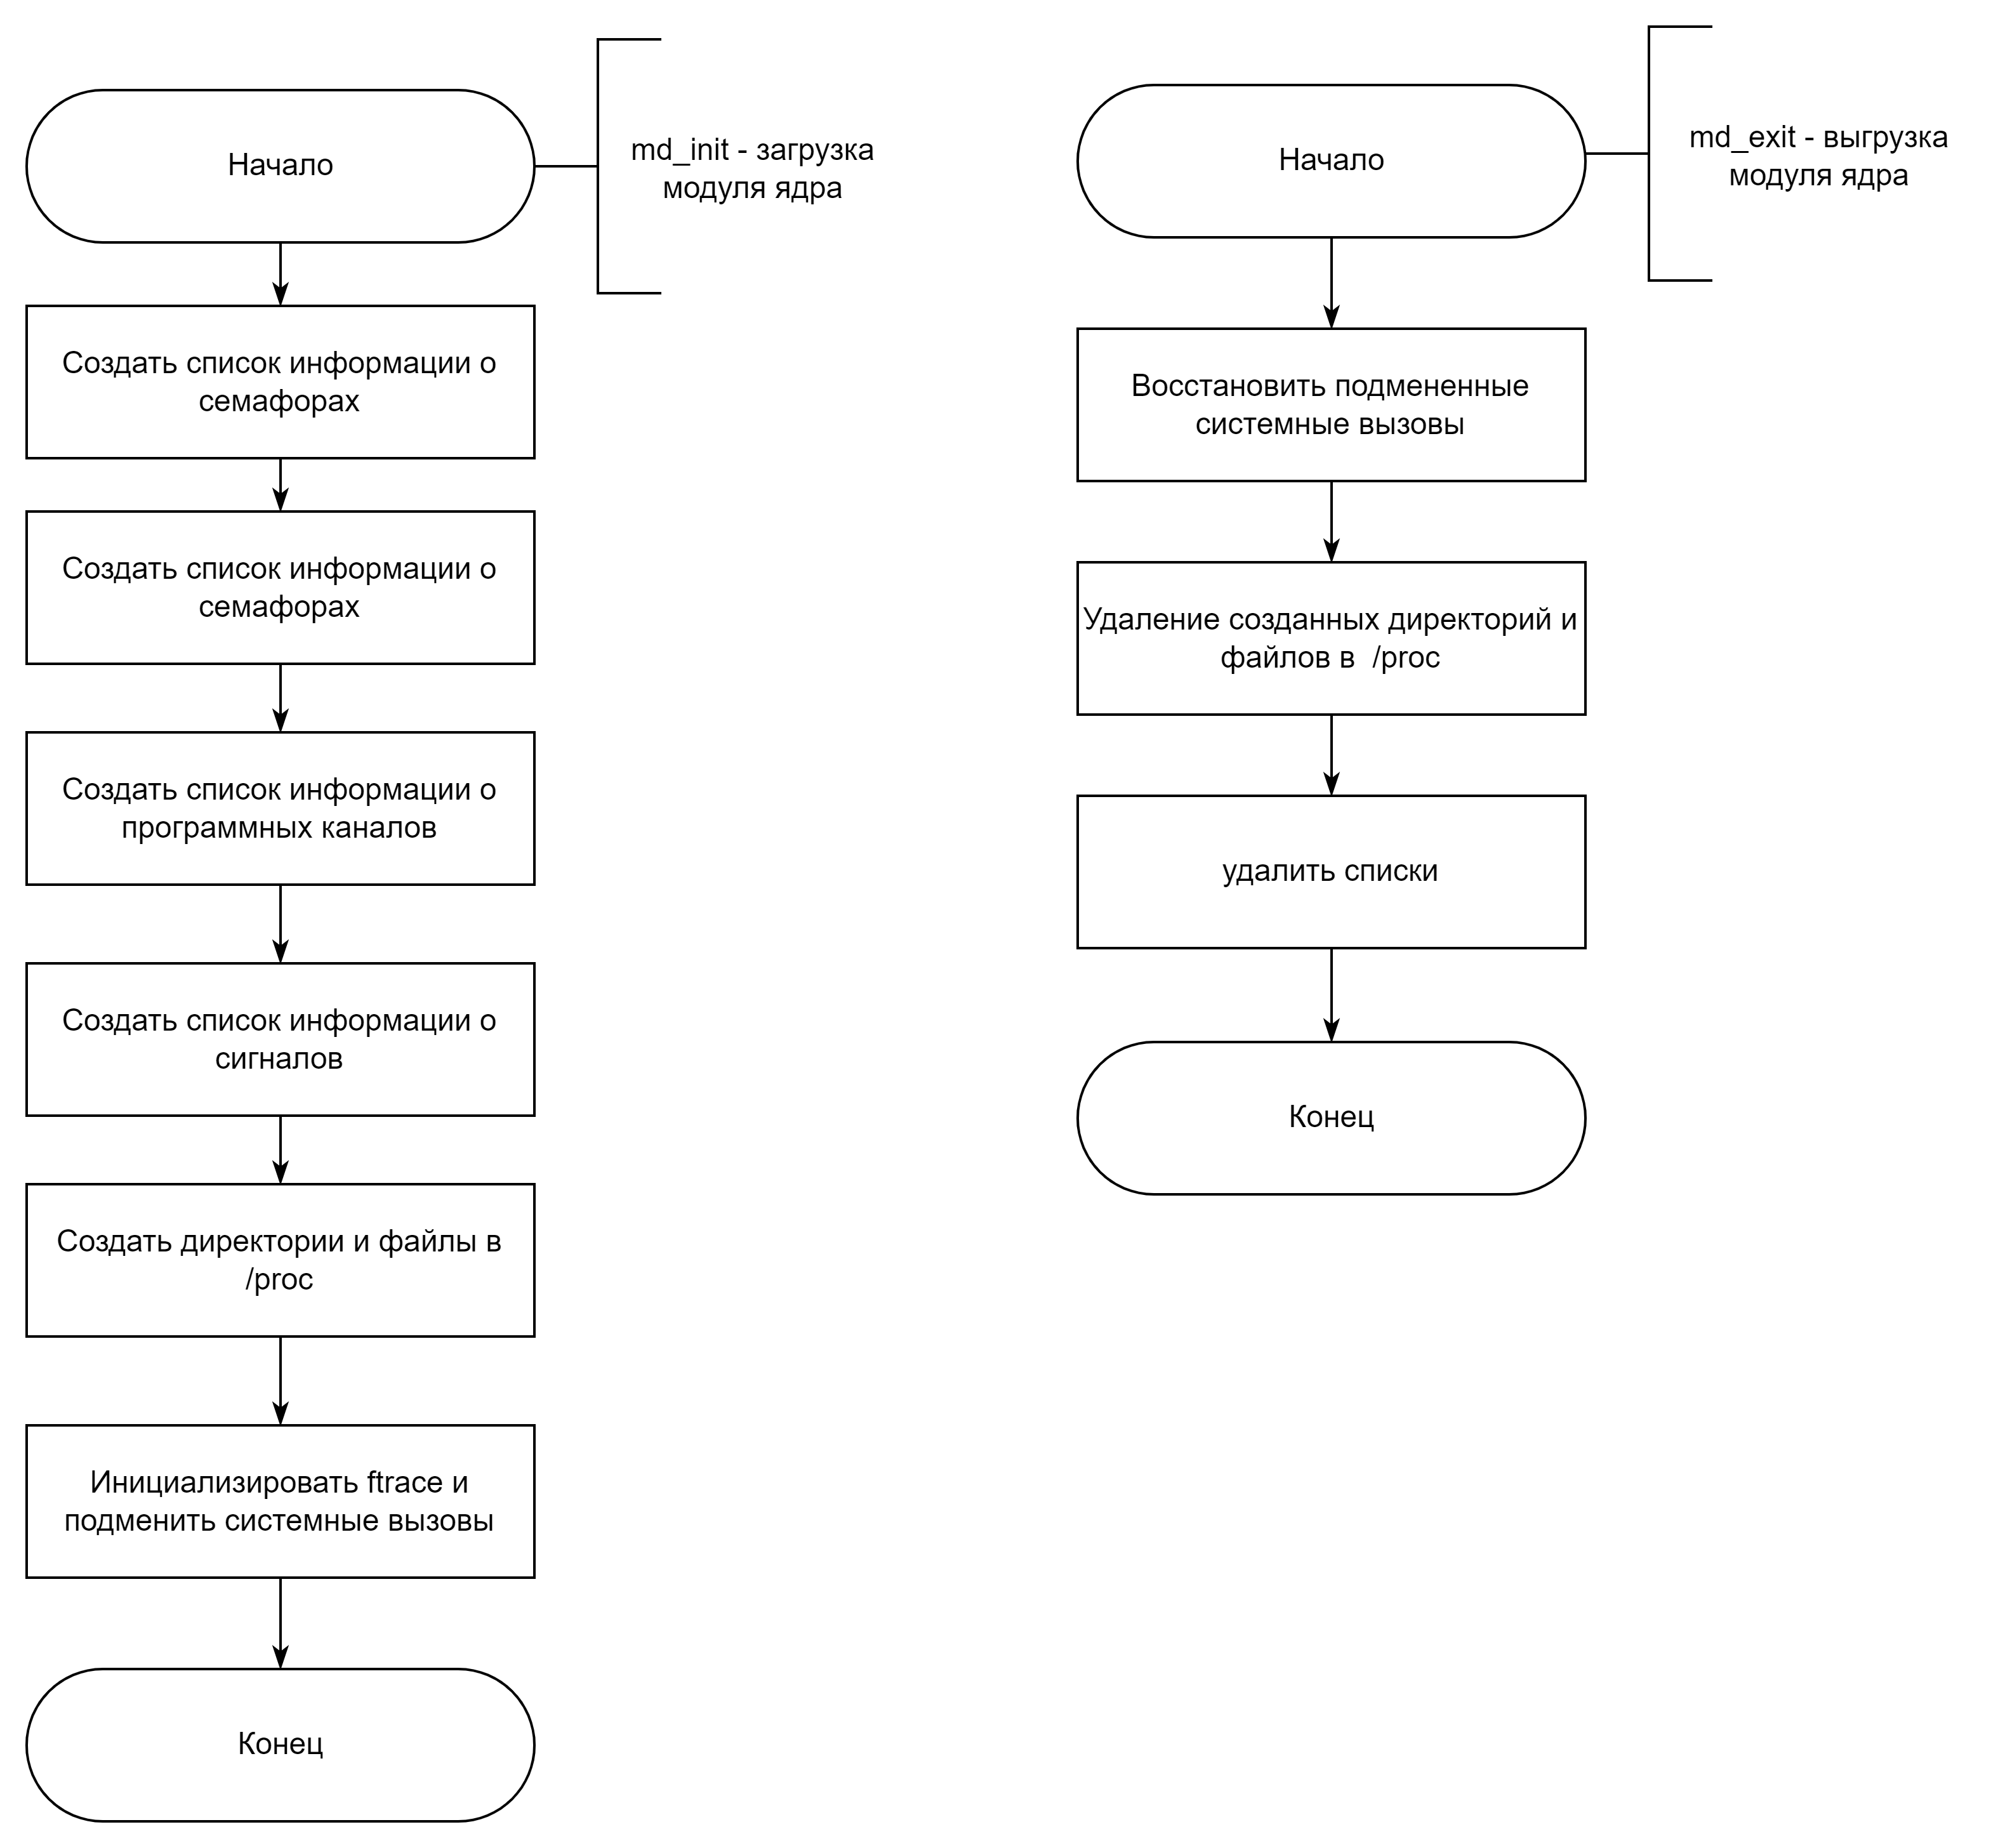
\includegraphics[height=0.6\textheight]{img/alg-md.png}
	\caption{Схемы алгоритмов загрузки и выгрузки модуля ядра}
	\label{img:alg:md}
\end{figure}

\clearpage

На риснуке~\ref{img:alg:proc} представлена схемы алгоритмов  создание и удаление директорий и файлов в \texttt{/proc}.

\begin{figure}[h]
	\centering
	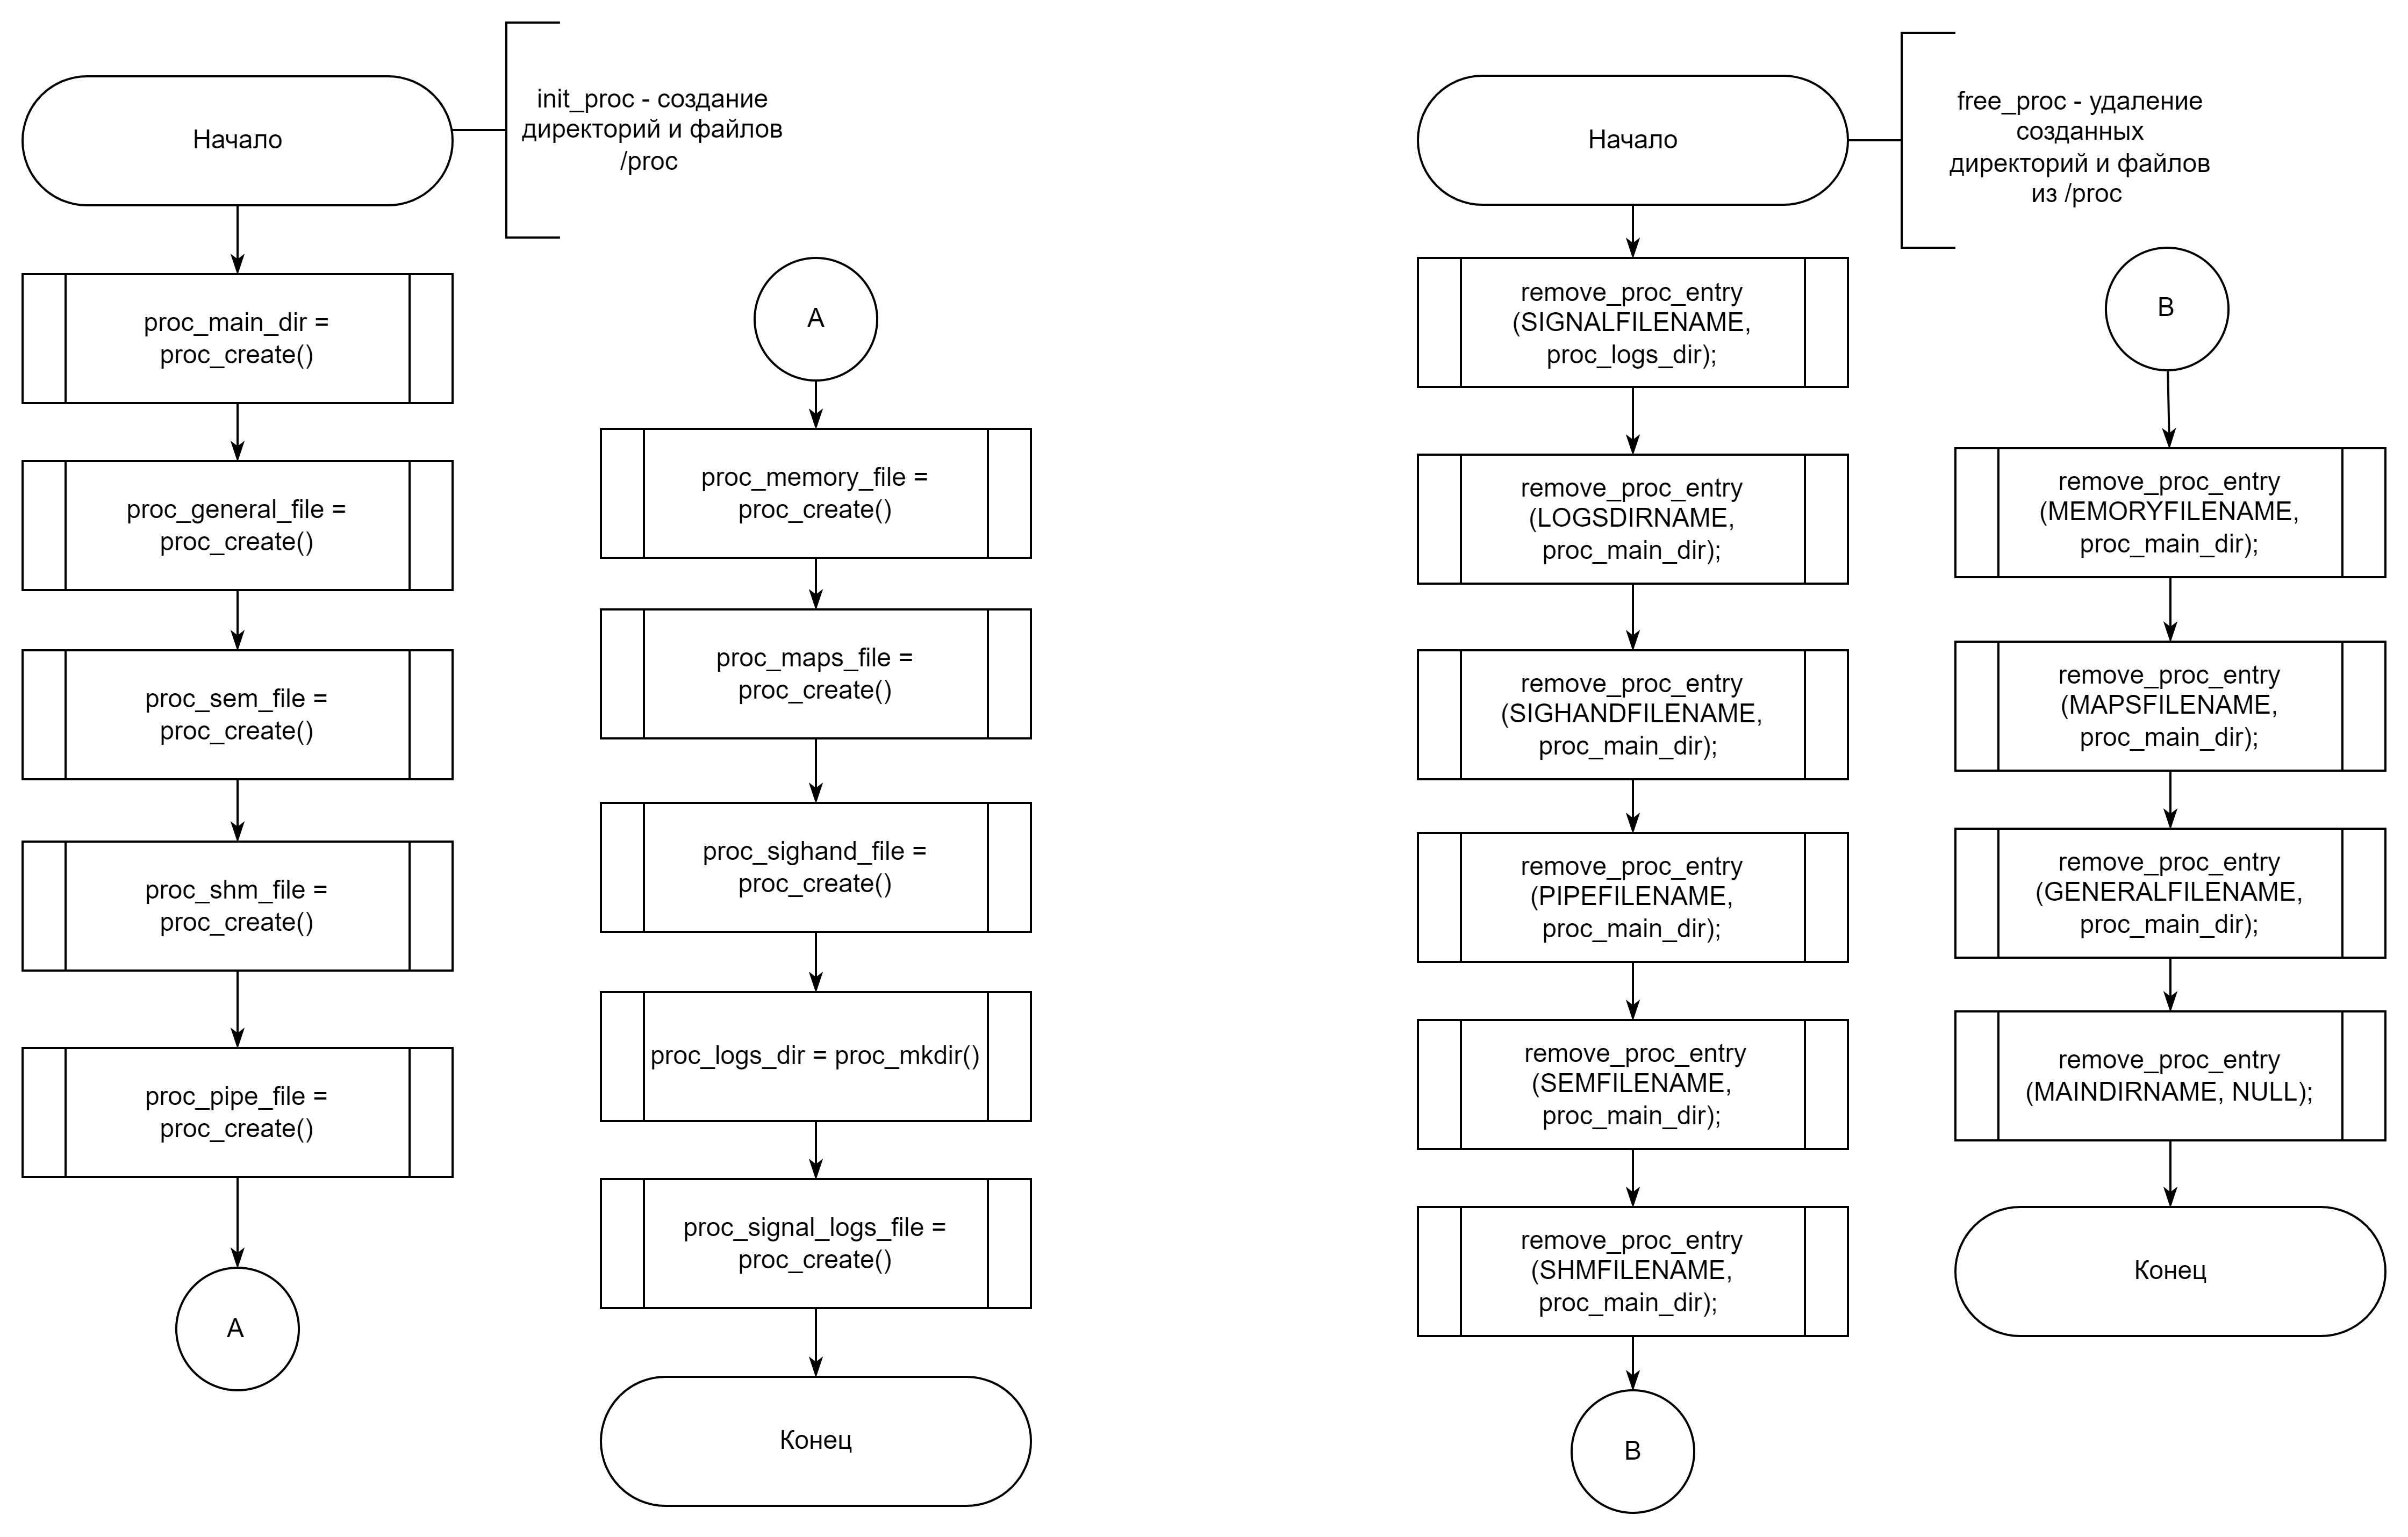
\includegraphics[height=0.4\textheight]{img/alg-proc.png}
	\caption{Схемы алгоритмов создание и удаление директорий и файлов в \texttt{/proc}}
	\label{img:alg:proc}
\end{figure}

При загрузке модуля ядра в \texttt{/proc} создаетсчя директория \texttt{monitroing} с файлами:
\begin{enumerate}
	\item \texttt{general} --- файл, который предоставляет информацию о проритете, времени выполнения и простоя, политики о процессов;
	\item \texttt{memory} --- файл, который предоставляет информацию о адресном пространстве процессов;
	\item \texttt{maps} --- файл, который предоставляет информацию о регионы адресного пространства процесса;
	\item \texttt{sighands} --- файл, который предоставляет информцию о назнчаченных обработчиках сигналов процессов. В данный файл необходимо записать pid процесса для получений данной информации;
	\item \texttt{sem} --- файл, который предоставляет информацию о семафорах;
	\item \texttt{shm} --- файл, который предоставляет информацию о сегментах разделямой памяти;
	\item \texttt{pipe} --- файл, который предоставляет информацию о программных каналах;
	\item \texttt{signals} --- файл, который предоставляет инфомацию о отправленных сигналах процессами.      
\end{enumerate}

На риснуке~\ref{img:alg:ftrace} представлена схема алгоритма перехвата системных вызовов.

\begin{figure}[h]
	\centering
	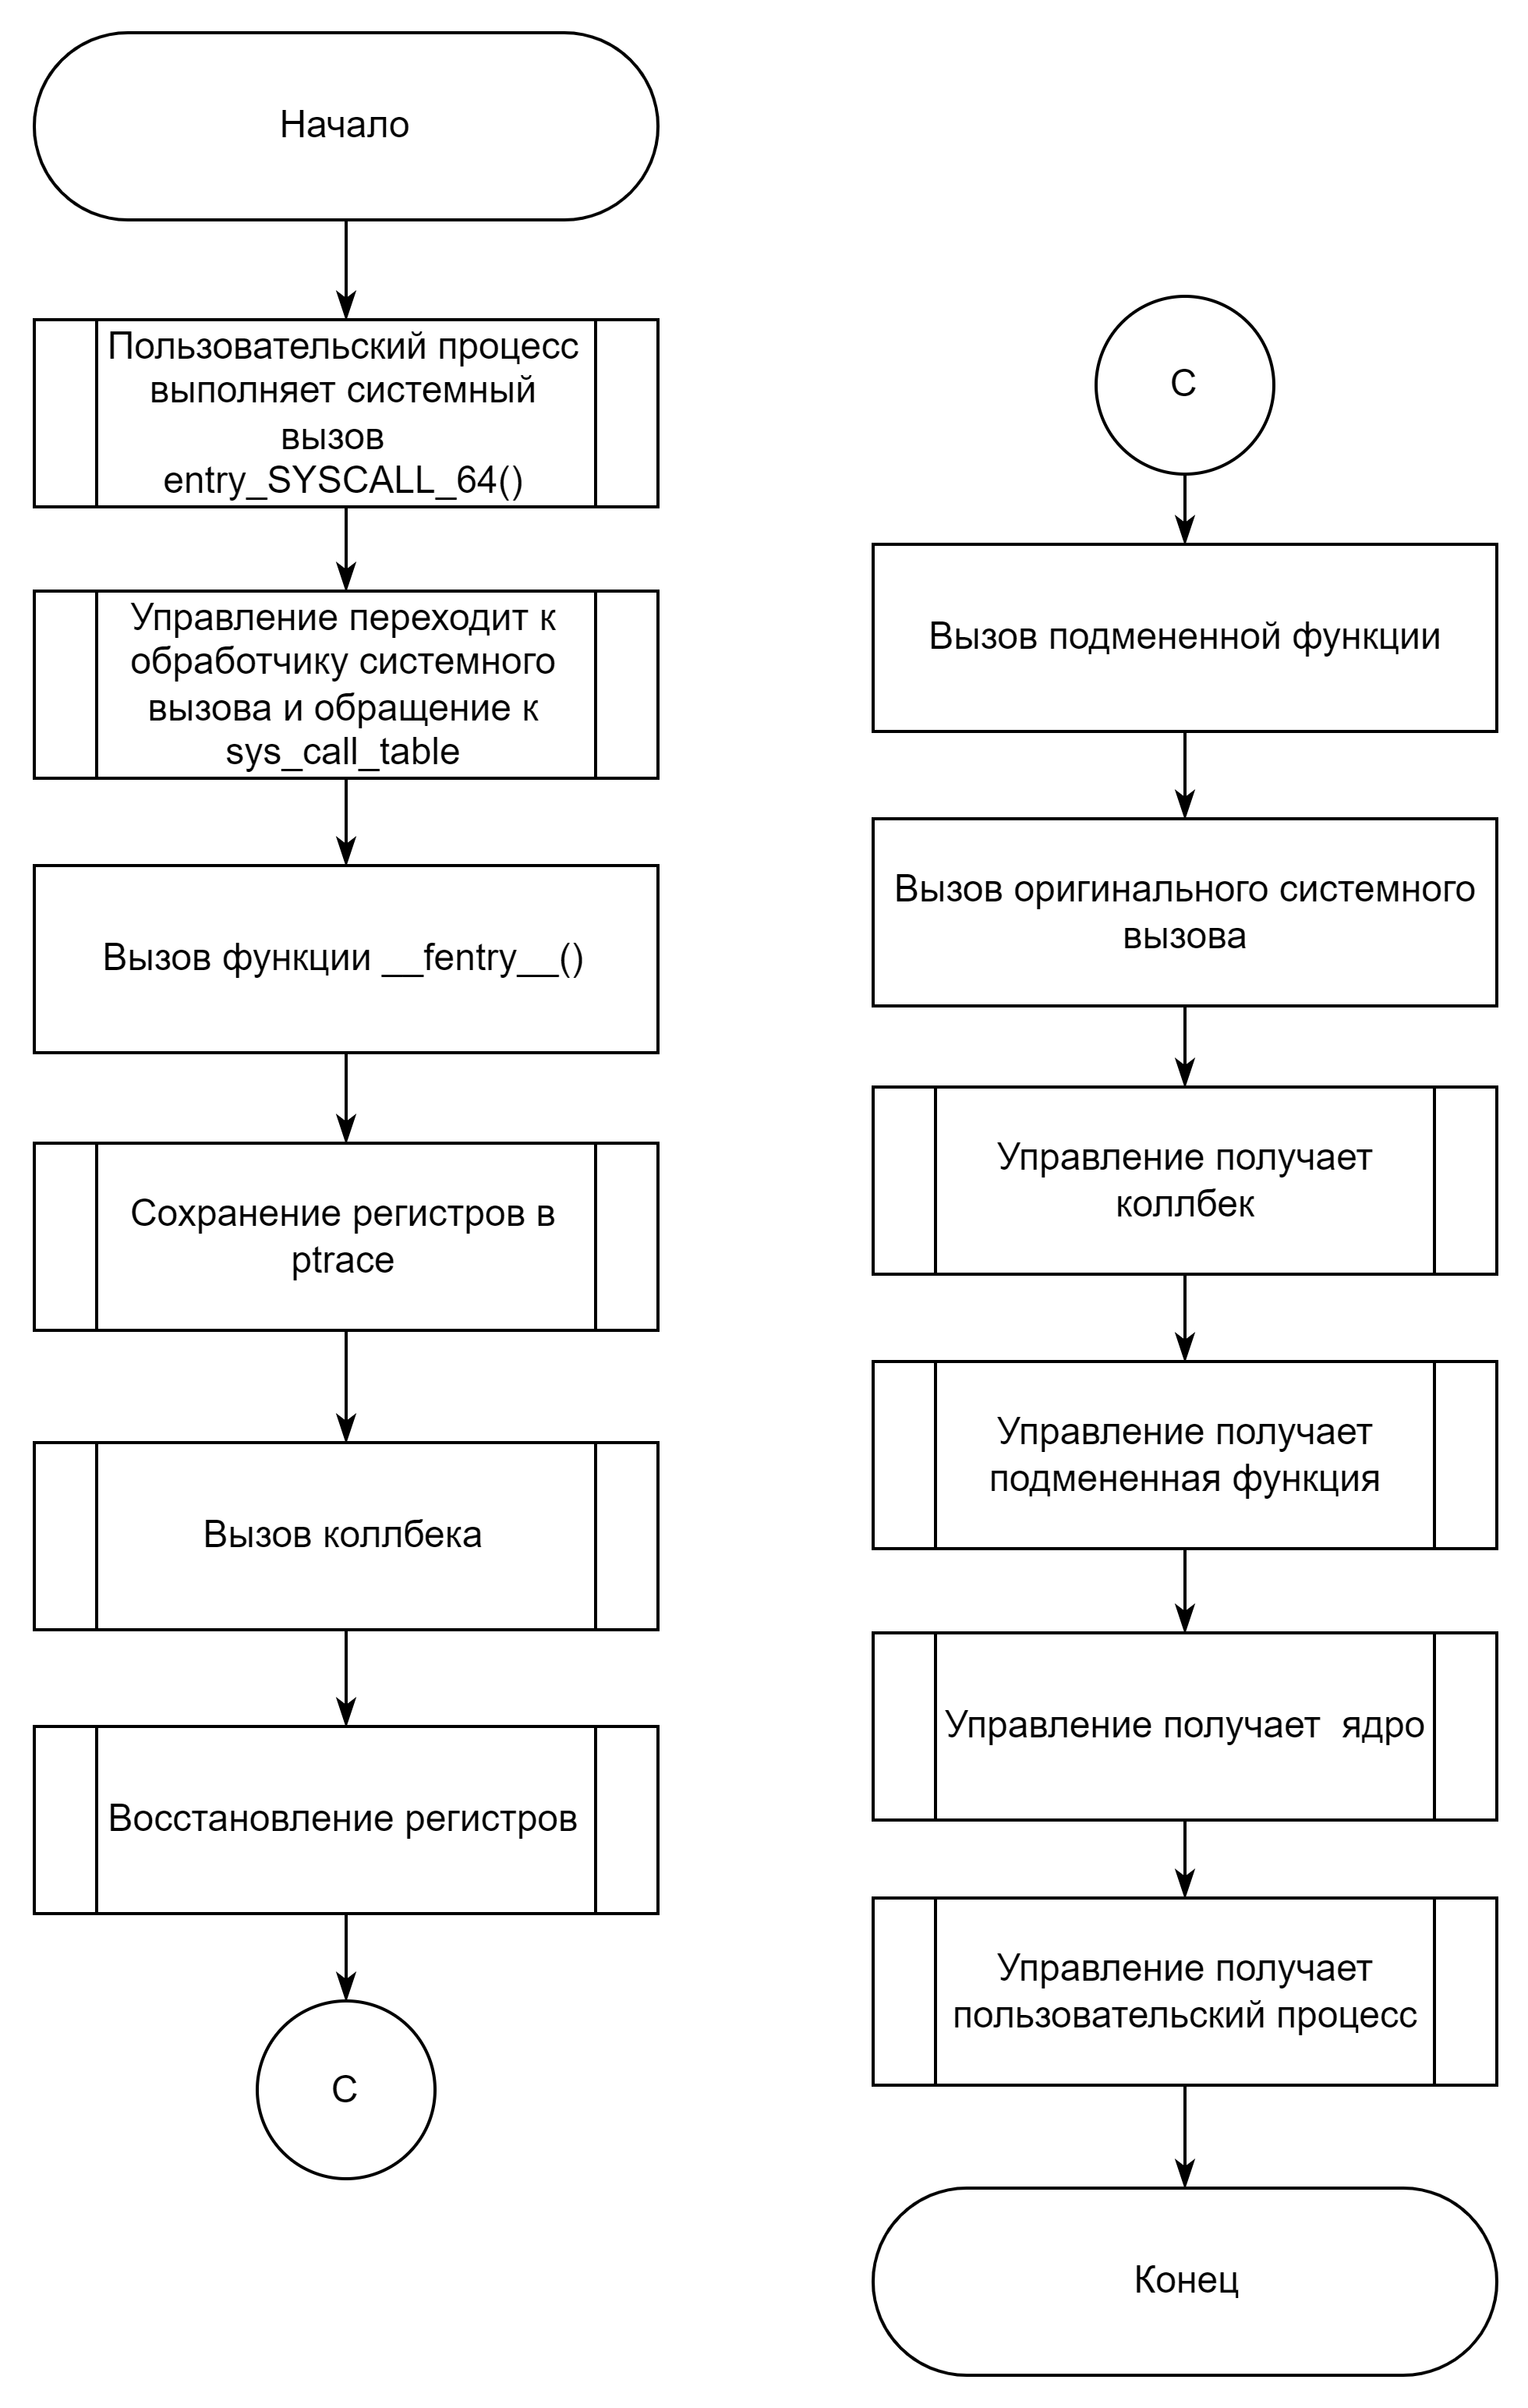
\includegraphics[height=0.6\textheight]{img/alg-ftrace.png}
	\caption{Схема алгоритма перехвата системного вызова}
	\label{img:alg:ftrace}
\end{figure}

Пользовательский процесс выполняет инструкцию \texttt{SYSCALL}. С помощью этой инструкции выполняется переход в режим ядра и управление передаётся низкоуровневому обработчику системных вызовов \newline \texttt{entry\_SYSCALL\_64()}. 
Управление переходит к обработчику системного вызова. Ядро передаёт управление функции \texttt{do\_syscall\_64()}. Эта функция обращается к таблице обработчиков системных вызовов \texttt{sys\_call\_table} и с помощью неё вызывает конкретный обработчик системного вызова.

Благодаря безусловному переходу, управление получает наша функция \texttt{hook\_sys\_clone()}, а не
оригинальная функция \texttt{sys\_clone()}. При этом всё остальное состояние процессора и памяти остаётся без изменений --- функция получает
все аргументы оригинального обработчика и при завершении вернёт
управление в функцию \texttt{do\_syscall\_64()}.

На риснуке~\ref{img:alg:general} представлена схема алгоритма чтения из файла \texttt{general}.

\begin{figure}[h]
	\centering
	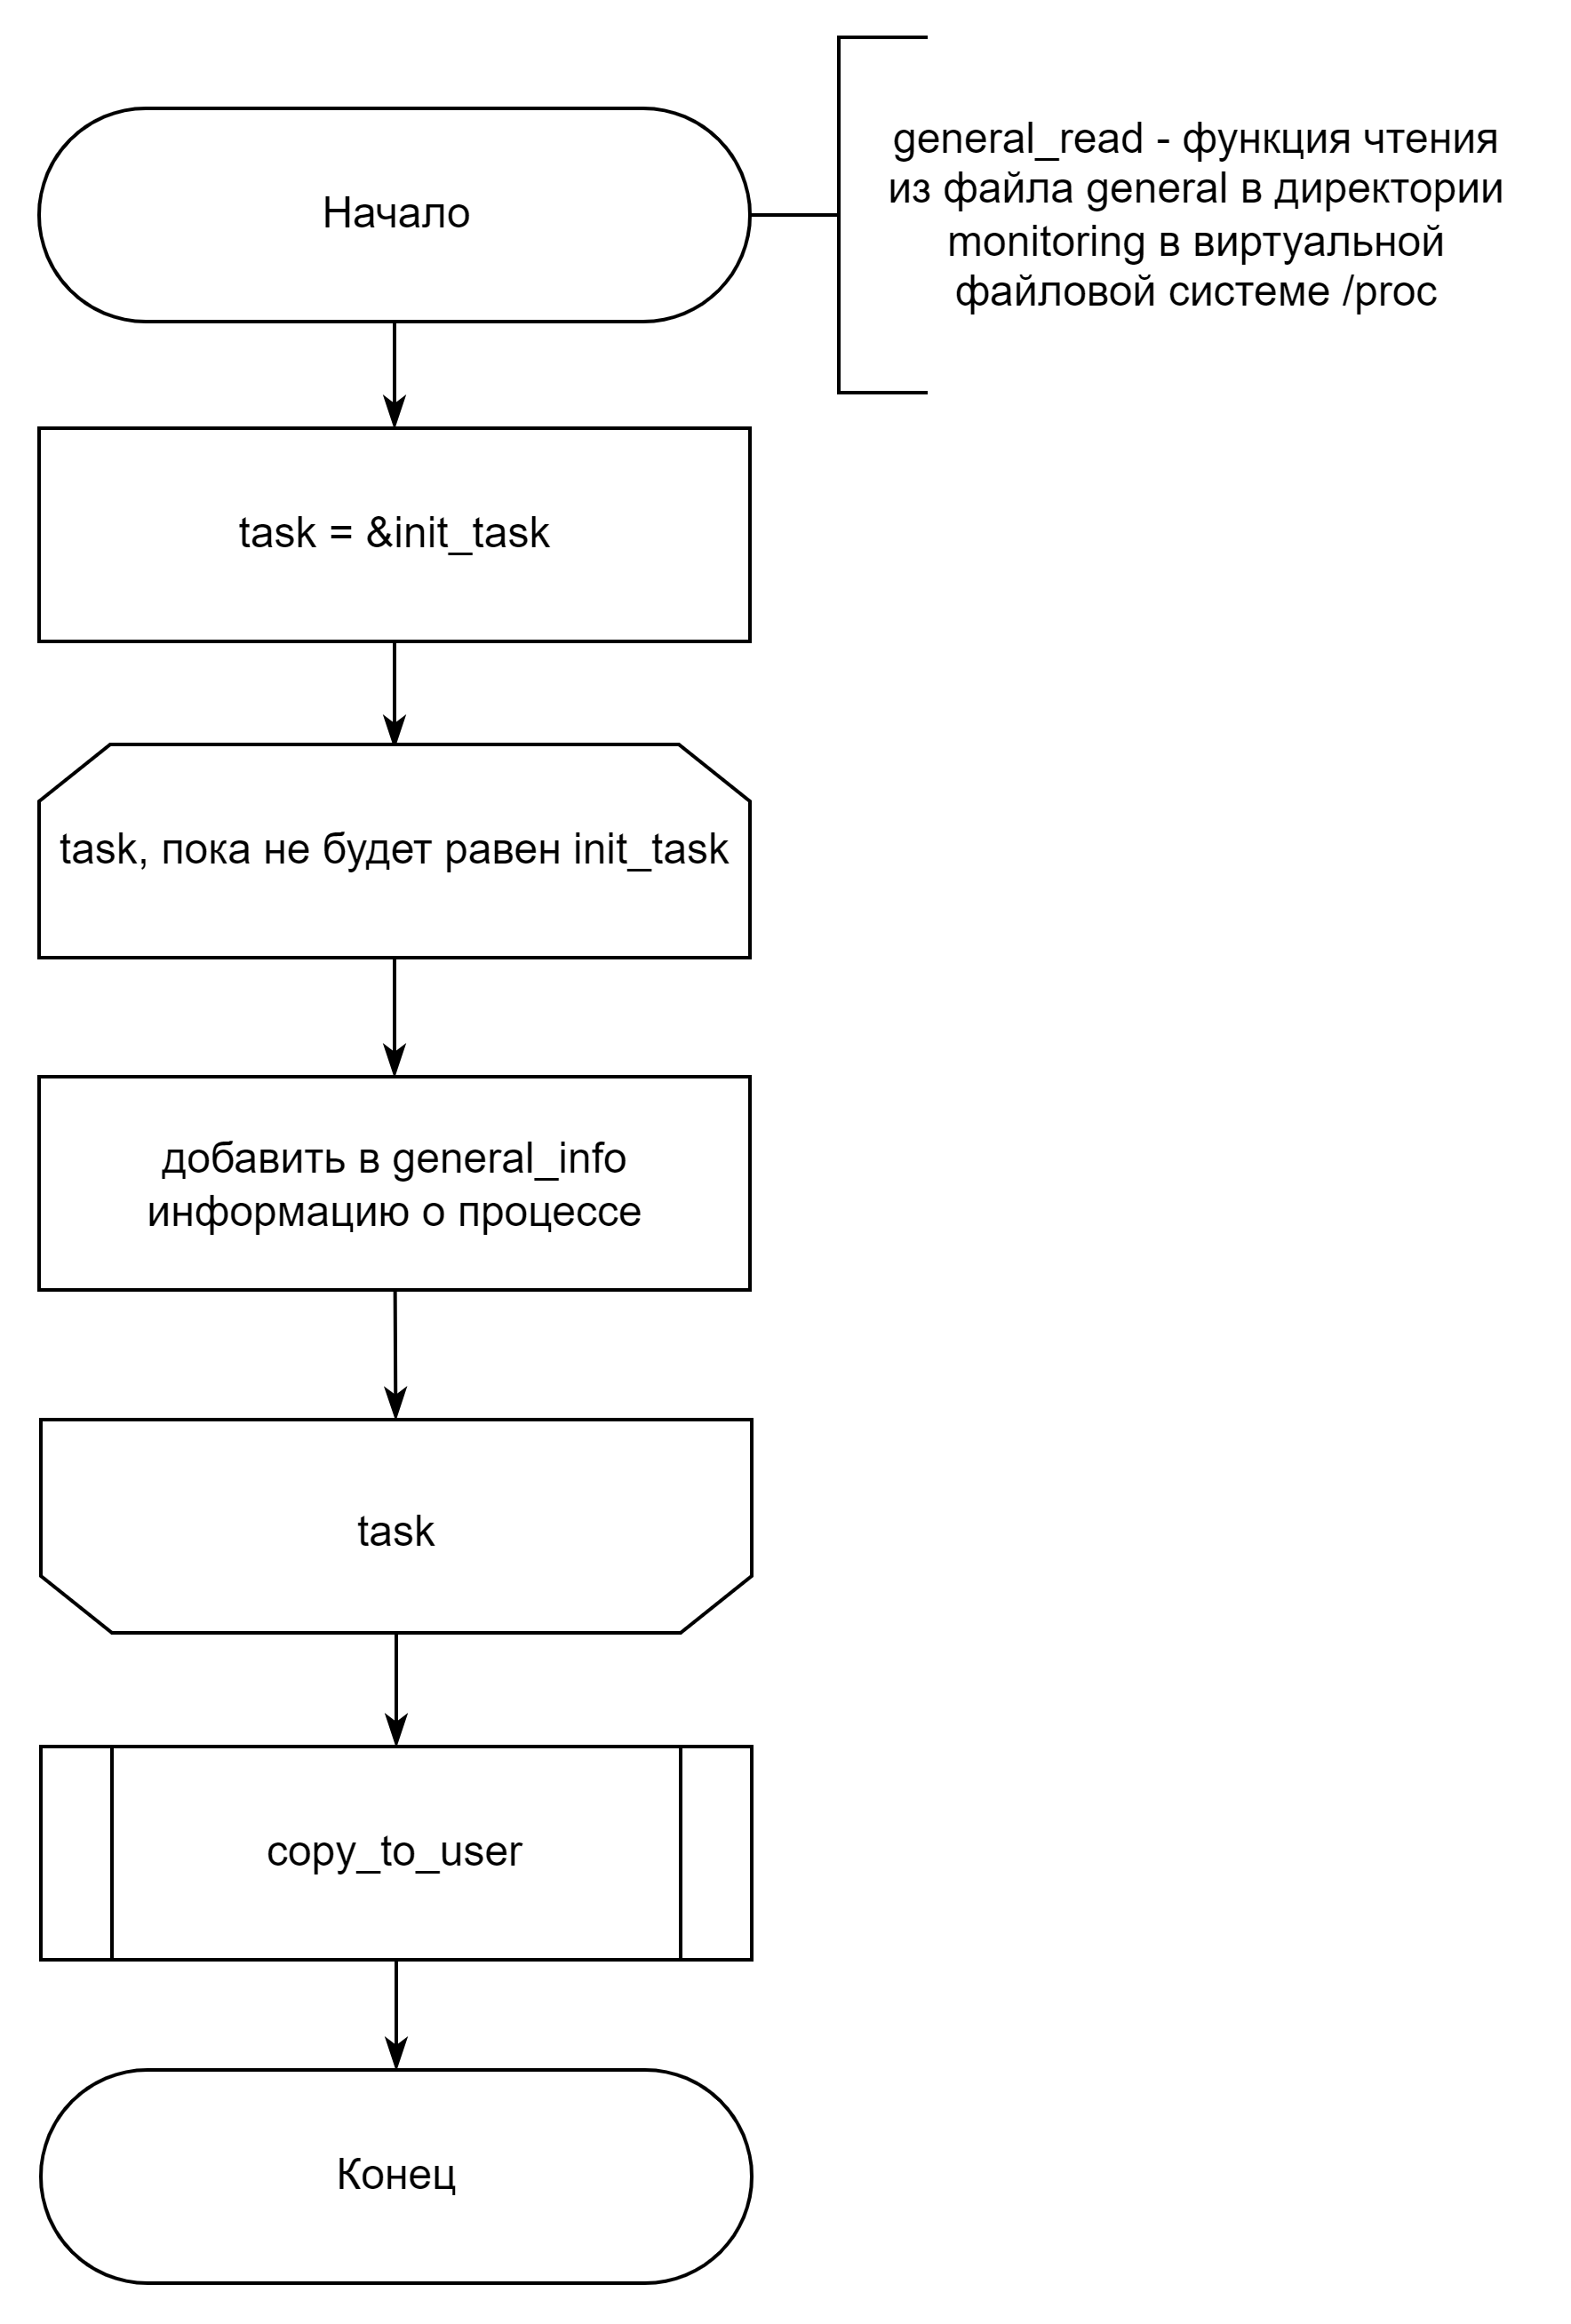
\includegraphics[height=0.6\textheight]{img/alg-general.png}
	\caption{Cхема алгоритма чтения из файла \texttt{general}}
	\label{img:alg:general}
\end{figure}

На риснуке~\ref{img:alg:sighand} представлена схема алгоритма чтения из файла \texttt{sighands}.

\begin{figure}[h]
	\centering
	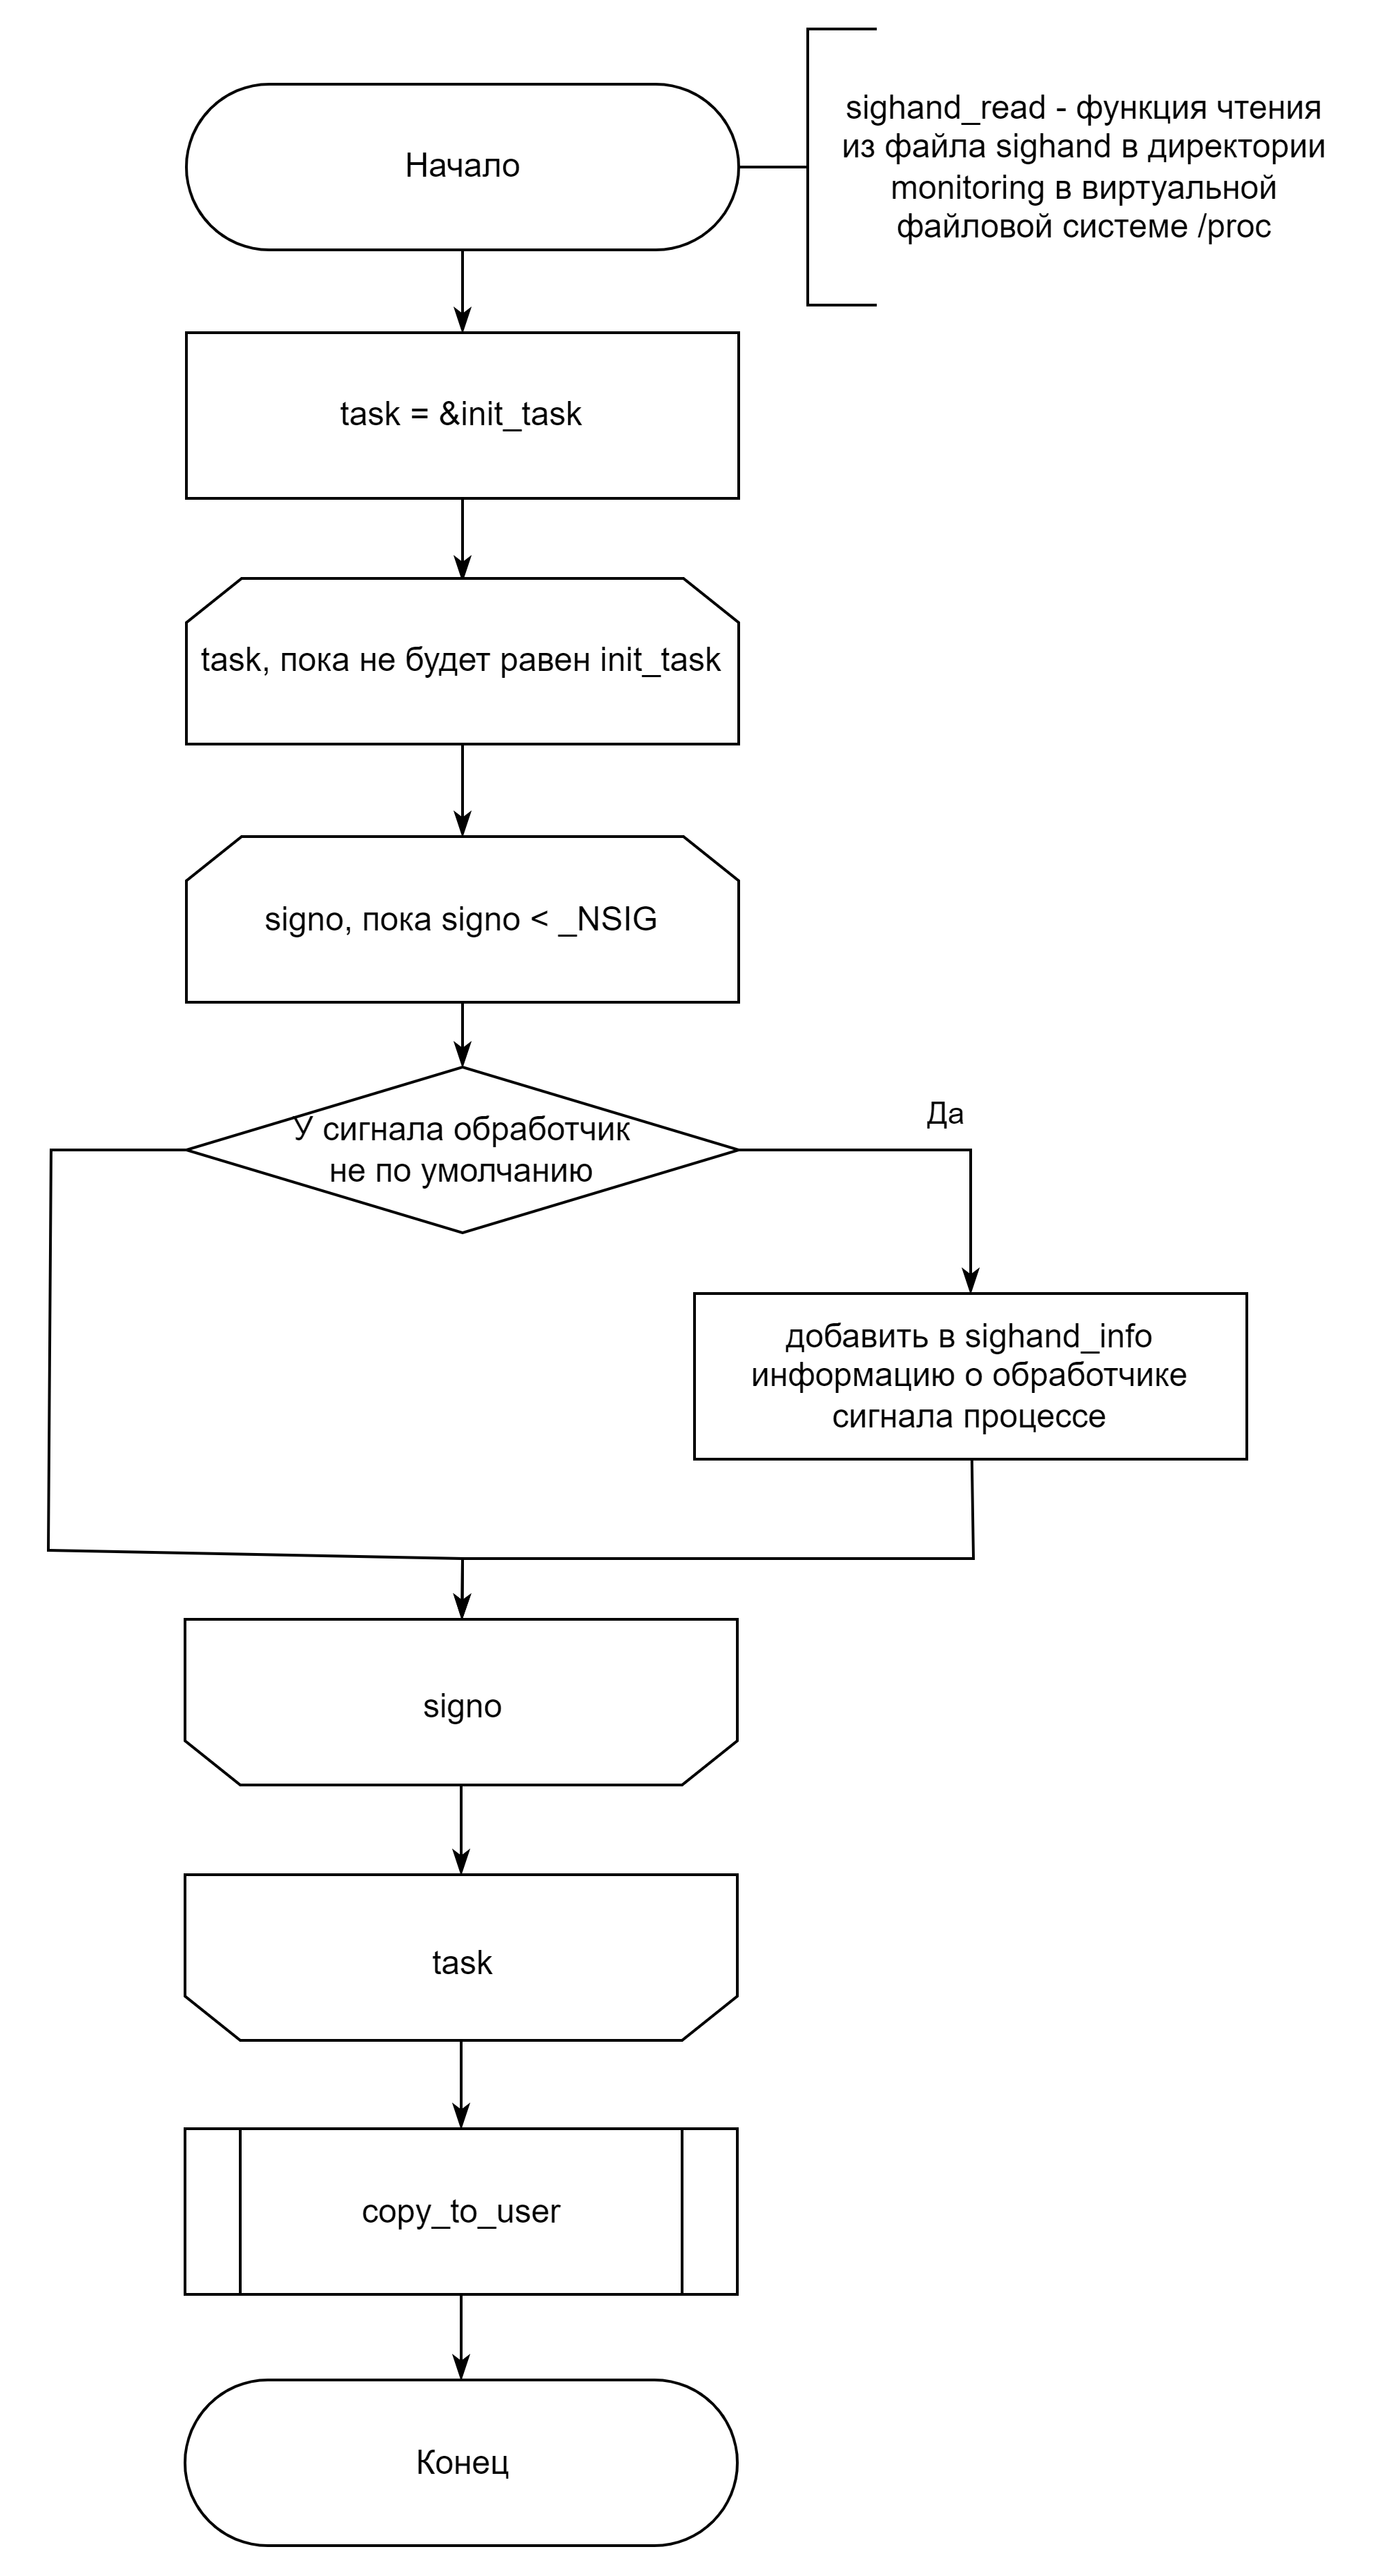
\includegraphics[height=0.7\textheight]{img/alg-sighand.png}
	\caption{Cхема алгоритма чтения из файла \texttt{sighands}}
	\label{img:alg:sighand}
\end{figure}

\clearpage

На риснуке~\ref{img:alg:shm-sem} представлена схемы алгоритмов чтения из файла \texttt{shm} и \texttt{sem}.

\begin{figure}[h]
	\centering
	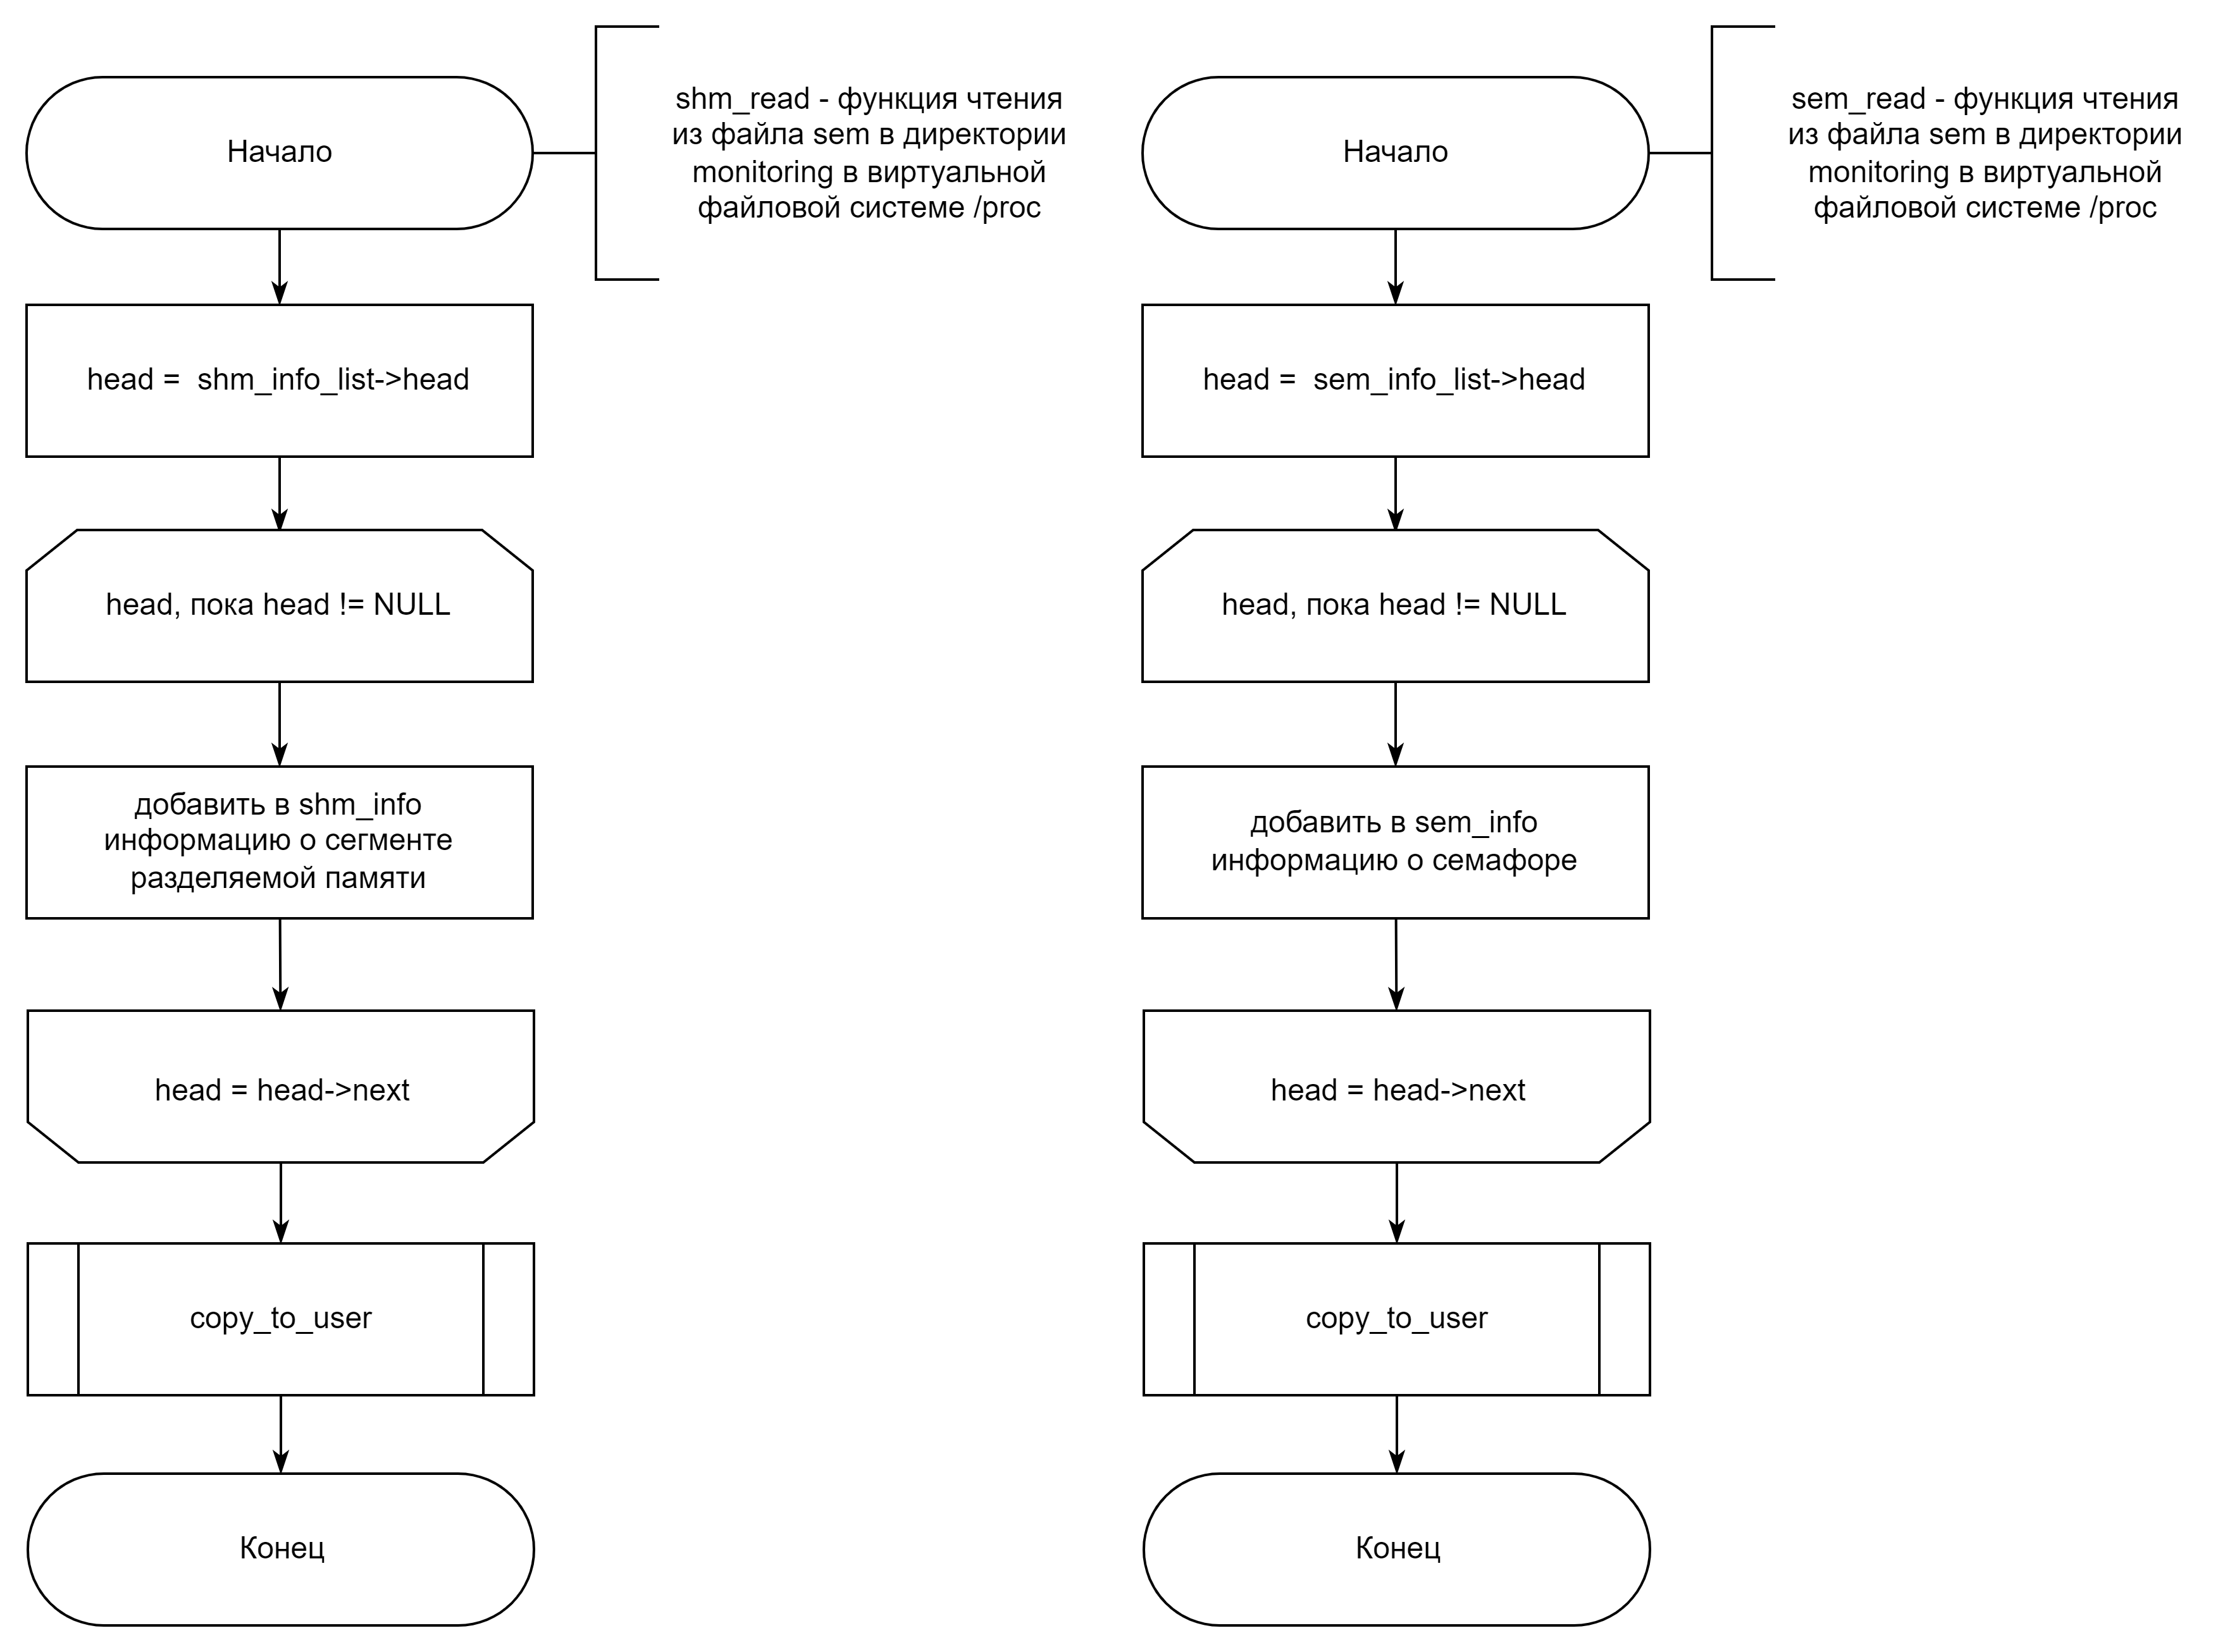
\includegraphics[height=0.5\textheight]{img/alg-shm-sem.png}
	\caption{Cхемы алгоритмов чтения из файла \texttt{shm} и \texttt{sem}}
	\label{img:alg:shm-sem}
\end{figure}

\clearpage

На риснуке~\ref{img:alg:hook-sem} представлена схемы алгоритмов подменяемой функции на примере \texttt{shmget()} и \texttt{shmctl()}.

\begin{figure}[h]
	\centering
	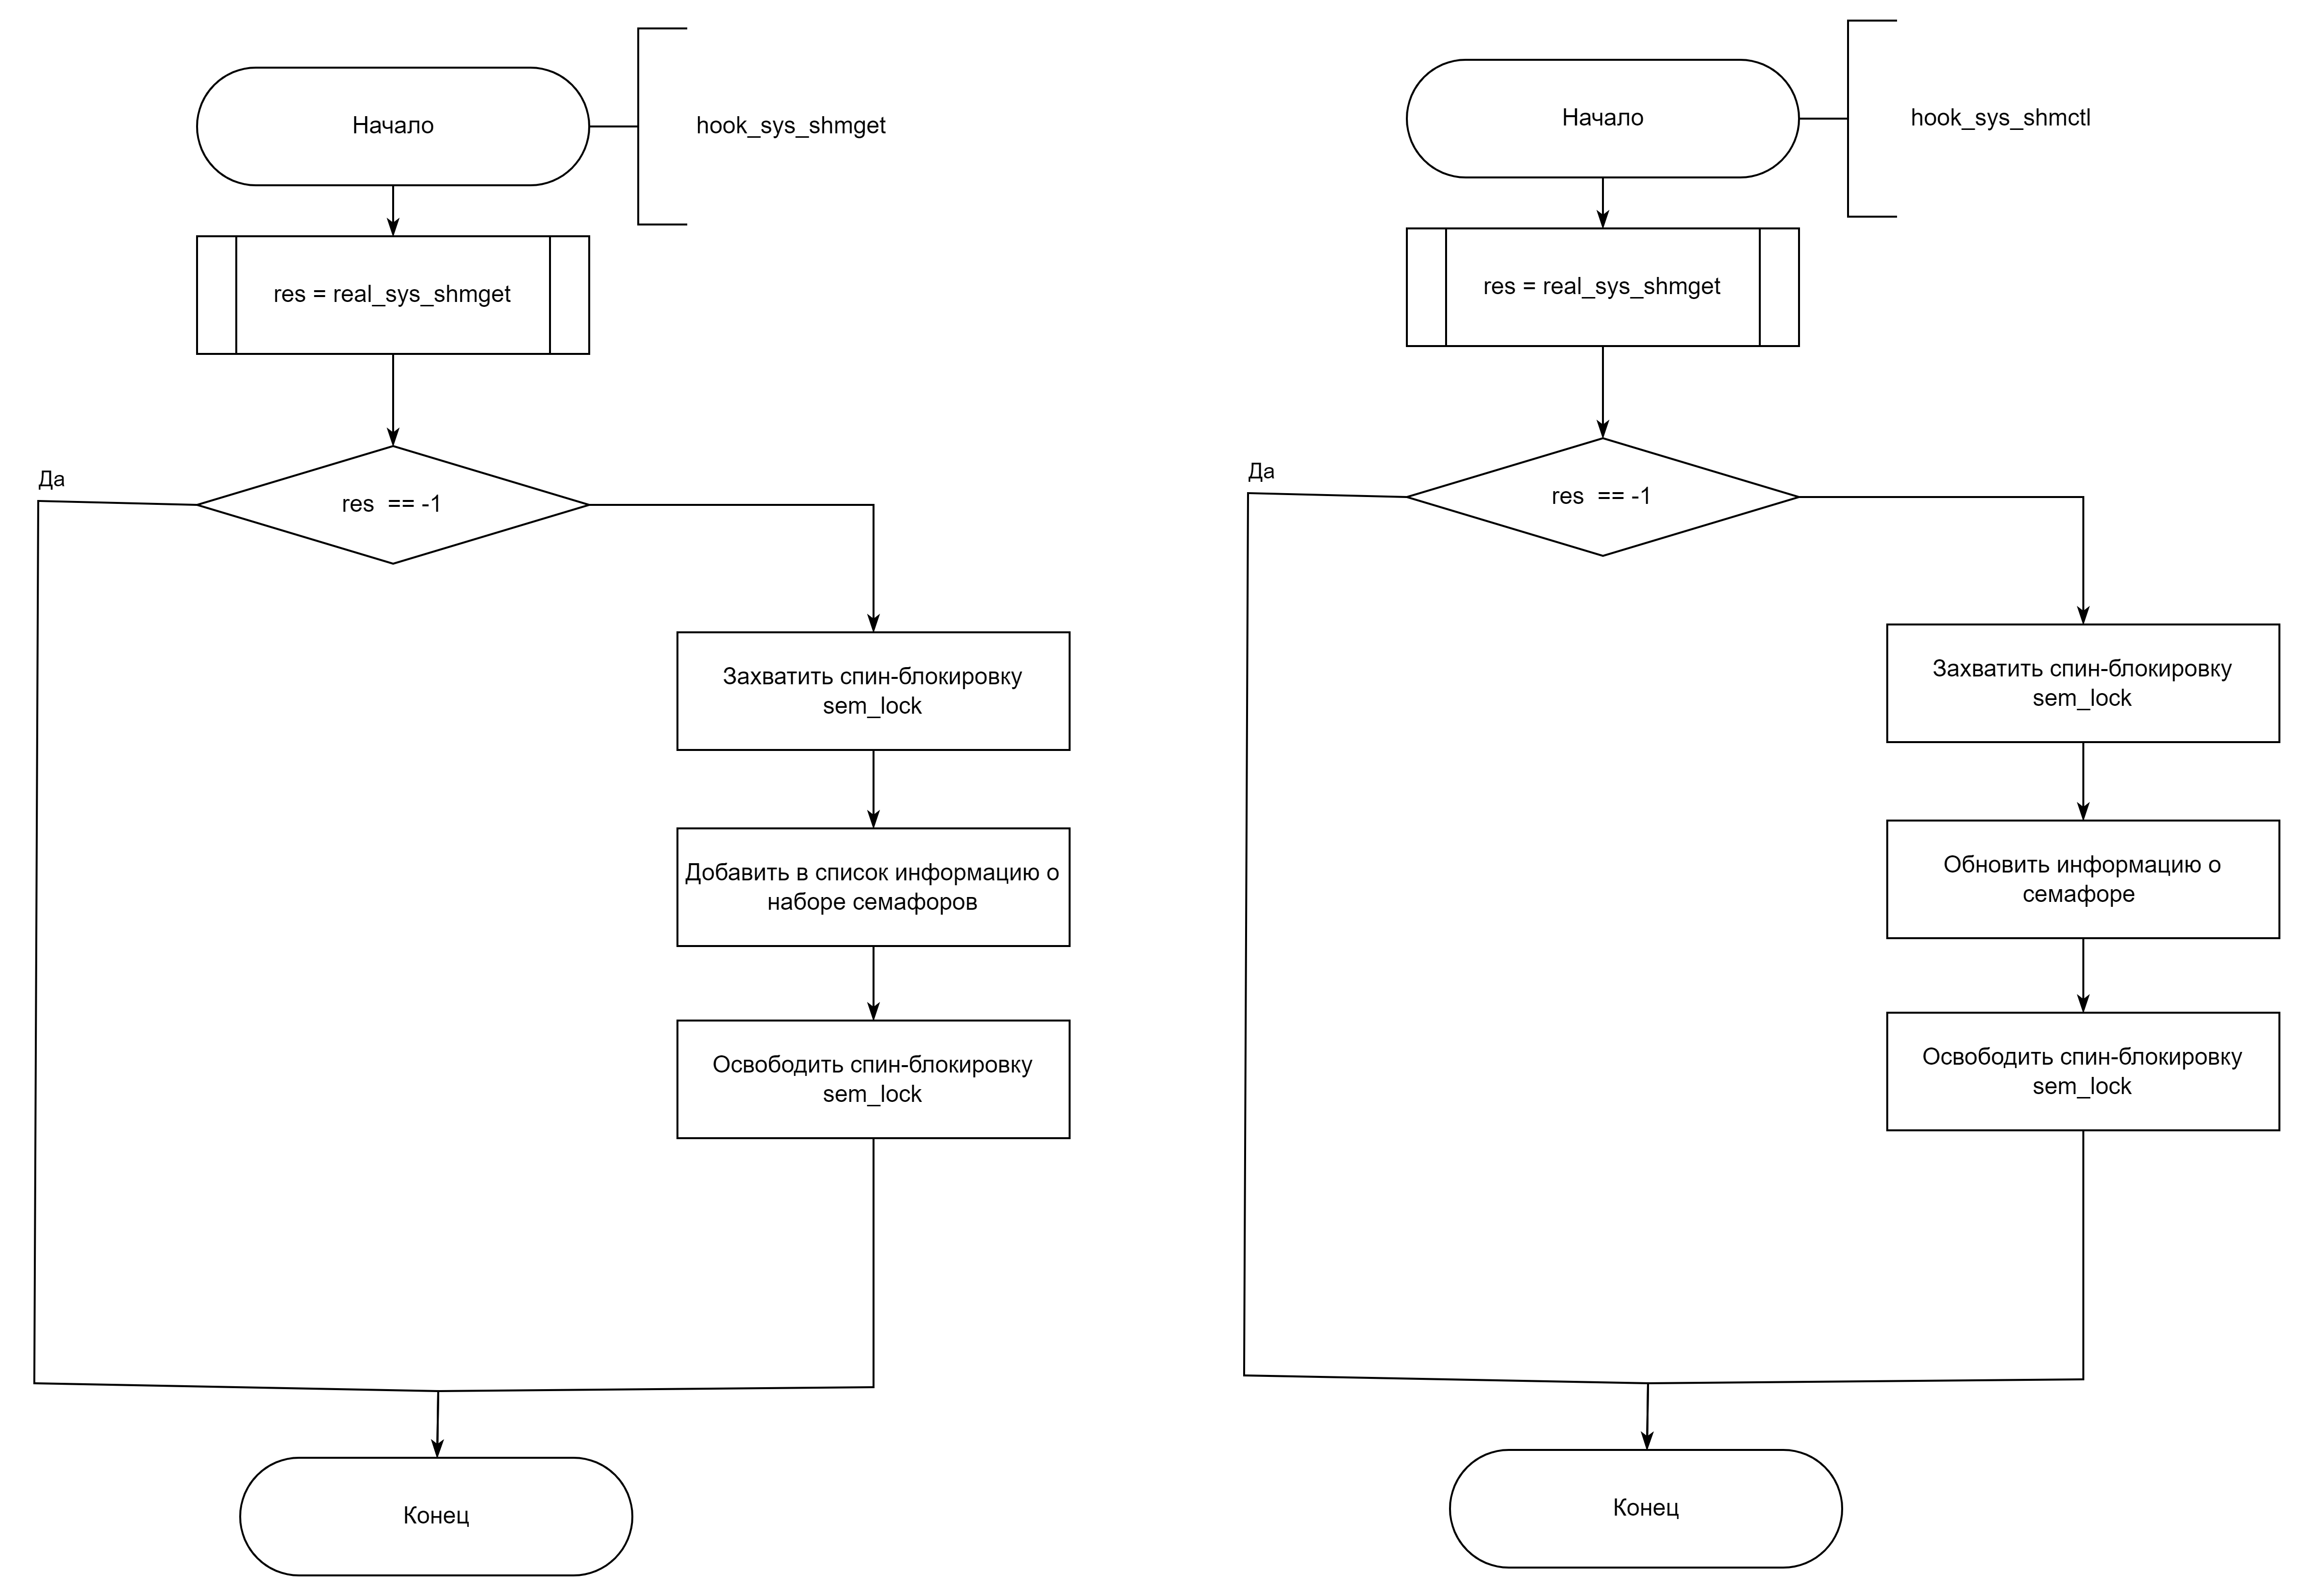
\includegraphics[height=0.4\textheight]{img/alg-hook-sem.png}
	\caption{Схемы алгоритмов подменяемой функции на примере \texttt{shmget()} и \texttt{shmctl()}}
	\label{img:alg:hook-sem}
\end{figure}